\section{Les différents type de classifieurs}

Il existe plusieurs types de classifieurs. Nous présentons içi quelques
classifieurs avec leurs avantages et inconvénients.

 \subsection{Méthode des K plus proche voisins (KNN)}

La méthode des 'K plus proche voisins' ou \textbf{k-Nearest Neighbors
KNN} en \nomenclature{KNN}{K-Nearest Neighbors}
anglais est une méthode de classification dans laquelle le modèle mémorise 
les observations de l’ensemble d’apprentissage pour la classification des 
données de l’ensemble de test.\cite{pradaig}

Son fonctionnement peut être assimilé à l’analogie suivante:
\textit{dis moi qui sont tes voisins, je te dirais qui tu es}.
Pour effectuer une prédiction, l’algorithme \textbf{K-NN} ne va pas calculer
un modèle prédictif à partir d’un training set(ensemble d'apprentissage) comme c’est le cas pour la 
régression logistique ou la régression linéaire. C'est pourquoi cet 
algorithme est qualifié de paresseux (Lazy Learning) car il n’apprend
rien pendant la phase d’entrainement. 

\subsubsection{Prédiction avec K-NN}
K-NN se base sur le jeu de donnée entier pour effectuer une prédiction. Pour 
un exemple qu'on souhaite prédire qui ne fait pas parti du jeu de données \cite{datascientist}
initiale, l’algorithme va chercher les \textit{K} instances du jeu de données les 
plus proches de notre exemple. Ensuite pour ces \textit{K} voisins, l'algorithme
se basera sur leurs étiquettes pour calculer l'étiquette de l'exemple que l'on
souhaite prédire.(figure~\ref{fig:knnfonctionnement})

\subsubsection{Similarité dans l'algorithme K-NN}
K-NN a besoin d’une fonction de calcul de distance entre deux exemples. Plus 
deux points sont proches l’un de l’autre, plus ils sont similaires et vice 
versa\cite{nagesh2019}.

Il existe plusieurs fonctions de calcul de distance, notamment, la distance 
euclidienne, la distance de Manhattan, la distance de Minkowski, celle de 
Jaccard, la distance de Hamming \ldots. La fonction de distance se choisit en
fonction des types de données qu’on manipule. Ainsi pour des données 
quantitatives (poids, salaires, taille, montant de panier éléctronique\ldots),
la distance euclidienne est un bon candidat. Quant à la distance de Manhattan,
elle est une bonne mesure quand les données ne sont pas de 
même type (age, sexe, longueur, poids\ldots).

\begin{figure}[h!]
  \begin{center}
    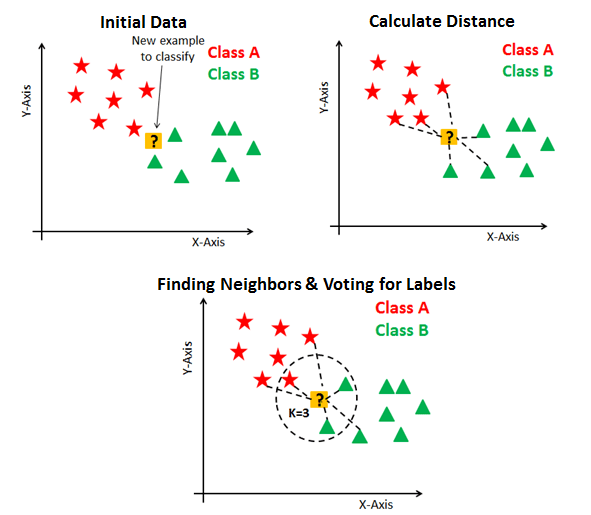
\includegraphics[width=12cm]{images/knn.png}
    \caption{Fonctionnement de l'algorithme K-NN.\label{fig:knnfonctionnement}}
  \end{center}
\end{figure}

\subsubsection{Choix de la valeur K}

Le choix de la valeur K varie en fonction du jeu de données. En règle générale, 
si K est petit, on sera sujet au sous apprentissage (underfitting). Par 
ailleurs, plus on utilise de voisins (K grand) la prédiction sera plus fiable. 
Toutefois, si on utilise K nombre de voisins avec K=N et N étant le nombre 
d’exemples, on risque d’avoir du overfitting et par conséquent un modèle qui se
généralise mal sur des observations qu’il n’a pas encore vu.

\subsubsection{Avantages}
\begin{description}
     \item{\textit{Absence d'apprentissage}}: Ce sont les échantillons pris en 
      considération, qui constituent le modèle.
    \item{\textit{Clarté des résultats: }} bien que la méthode ne produise pas de 
        règle explicite, la classe attribuée à un exemple peut être expliquée en
        exposant les plus proches voisins qui ont imposé cette attribution.
       \item{\textit{Grand nombre d'attributs:}} la méthode permet de traiter des
          problèmes avec un grand nombre d'attributs. Cependant, plus le nombre 
          d'attributs est important, plus le nombre d'exemples doit être grand.
      \end{description}

\subsubsection{Inconvénients}
\begin{description}
   \item{\textit{Sélection des attributs pertinents:}} Pour que la notion de proximité
    soit pertinente, il faut que les exemples couvrent bien l'espace et soient 
    suffisamment proches les uns des autres. Si le nombre d'attributs pertinents est
    faible relativement au nombre total d'attributs, la méthode donnera de mauvais 
    résultats.
   \item{\textit{Le temps de classification:}} Si la méthode ne nécessite pas 
    d'apprentissage, tous les calculs doivent être effectués lors de la classification 
    d'un nouvel exemple.
  \item{\textit{Définir les distances et nombres de voisins:}} Les performances de la 
      méthode dépendent du choix de la distance, du nombre de voisins et du mode de 
      combinaison des réponses des voisins.
  \end{description}

\subsection{Les réseaux de neurones}
Les réseaux de neurones sont inspirés de la structure neurophysiologique des
neurones. En règle générale, un réseau de neurones repose sur un grand nombre de
processeurs opérant en parallèle et organisés en tiers(couches). La première
couche reçoit les entrées d’informations brutes, un peu comme les nerfs optiques
de l’être humain lorsqu’il traite des signaux visuels. Par la suite, chaque
couche  reçoit les résultats de la couche précédente.
On retrouve le même processus chez l’Homme, lorsque les neurones reçoivent des
signaux en provenance des neurones proches du nerf optique. La dernière couche,
quant à elle, produit les résultats du système.

\subsubsection{Les différents cas d'usage}

Les réseaux de neurones sont beaucoup utilisés dans la reconnaissance d'écriture
manuscrites, la transcription \og speech-to-text \fg ou encore dans la
prévision des marchés financiers ou trading algorithmique.

Ils peuvent aussi être utilisé pour la reconnaissance faciale, la prédiction
météo, la détection de cancer sur les imageries médicales. De manière générale,
les réseaux de neurones excellent pour la reconnaissance de patterns.

\subsubsection{Avantages}
\begin{description}
  \item{\textit{Classification efficace :}} le calcul d'une sortie à partir d'un 
    vecteur d'entrée est un calcul très rapide.
  \item{\textit{Les données réelles :}} les réseaux traitent facilement les données 
      réelles "préalablement normalisées" et les algorithmes sont robustes au bruit.
  \end{description}

\subsubsection{Inconvénients}
\begin{itemize}
  \item Déterminer l’architecture du réseau est complexe et les
    paramètres sont difficiles à interpréter (boite noire).
    \item L'échantillon nécessaire à l'apprentissage doit être
      suffisamment grand et représentatif des sorties attendues.
  \end{itemize}

\subsection{Support Vector Machine (SVM)}
Les Support Vector Machine ou Machine à Vecteur de Support constituent une 
technique d’apprentissage supervisée. Elles ont été inventées par Boser, 
Guyon et Vapnik \cite{10.1145/130385.130401} et présentées pour la première
fois à la conférence Computational Learning Theory (COLT) de 1992.
Grâce à ses performances \cite{Cortes1995}, cette technique a ouvert un domaine de 
recherche très actif et un grand éventail d’applications. Les SVM utilisent
une approche géométrique pour classer les données en deux catégories.

En considérant les données comme des vecteurs, les SVM construisent un plan(une
frontière) qui sépare les données dans chacune des catégories.
Une fois la frontière de décision construite(Hyperplan) la
SVM\nomenclature{SVM}{Support Vector Machine} sera capable de
classer de nouvelles données en observant de quel côté de la frontière elles
tombent, et en leur assignant la catégorie correspondante.

L'idée est donc de rechercher le meilleur hyperplan qui sépare linéairement deux
classes, tout en les repoussant aux maximum. Lors de la phase d'apprentissage,
le svm cherche à maximiser la marge entre les deux classes d'apprentissage. Ce
qui lui procure une grande capacité de généralisation pendant la phase de test.

Les machines à vecteurs de support ont été appliquées dans des domaines comme
la reconnaissance automatique des visages et des gestes \cite{840634}, la
prédiction des mouvement de la bourse\ldots \cite{HUANG20052513}.

 Les domaines dans lesquels, elles sont les plus efficace sont: la reconnaissane d'objet et de
 d'image \cite{788125} et la catégorisation de texte \cite{6990940}



\begin{figure}[h!]
  \begin{center}
    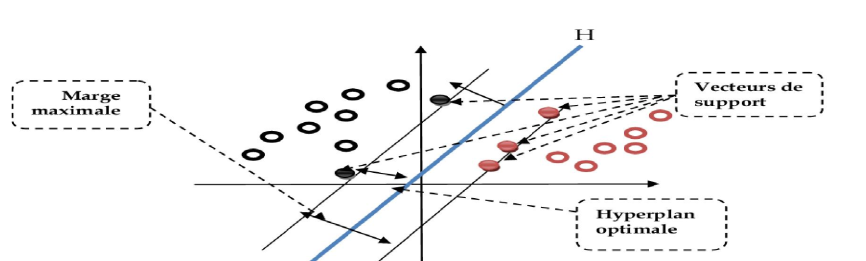
\includegraphics[width=14cm]{images/marge.png}
      \caption{Machine à vecteurs de support .\label{fig:marge}}
  \end{center}
\end{figure}

\subsubsection{Avantage}
\begin{itemize}
  \item Grâce à leurs fondements mathématiques solides, les SVM possèdent donc
    une grande précision de prédiction
  \item les SVM fonctionnent bien sur de petits jeux de données
  \item Décision rapide. La classification d’un nouvel exemple consiste à voir le signe de
    la fonction de décision f(x). 
\end{itemize}

\subsubsection{Inconvénient}
Les SVM ne conviennent pas à des jeux de données très volumineux car le temps
d'entrainement est très long.

  Les SVM effectuent une classification binaire d’où la nécessité d’utiliser 
l’approche un-contre-un pour construire un classifieur multiclasse.
Une grande quantité d’exemples en entrées implique un calcul matriciel important.
Le temps de calcul est élevé lors d’une régularisation des paramètres de la 
fonction noyau. 

Les SVM sont moins efficaces sur les jeux de données contenant
du bruits et beaucoup d’outliers

 \subsection{Les arbres de décisions}
Un arbre de décision est un outil d’aide à la décision qui permet de
répartir une population d’individus en groupes homogènes selon des attributs
discriminants en fonction d’un objectif fixé. Il permet d'émettre des
prédictions sur le problème par réduction niveau après niveau du domaine.

Les arbres de décision sont facilement interprétables, toutefois, leur capacité de
prédiction est presque toujours dépassée par les autres modèles de classication. 
Cette caractéristique a limité son utilisation. Au début des années 2000,
ils ont été repris comme élément de base d'une nouvelle méthode de
classification, appelée la forêt aléatoire de décision.

Cette nouvelle technique utilise de manière combinée les arbres de
décision et la théorie statistique pour réduire la variance du classeur en calculant la
moyenne d'un ensemble d'arbres de décision en générant des classeurs avec une très
bonne capacité de prévision. Nous les présenterons plus largement dans les
prochaines sections.

\subsubsection{Avantages}
\begin{description}
   \item{\textit{Adaptabilité aux attributs de valeurs manquantes :}} les
    algorithmes peuvent traiter les valeurs manquantes (exemples contenant
    des champs non renseignés) pour l'apprentissage, mais aussi pour la 
    classification.
  \item{\textit{Modèle white-box }} D'un arbre de décision, il
    est possible de générer des règles permettant d'expliquer ou de comprendre le
    résultat d'une classification. le résultat est facile à conceptualiser, 
    à visualiser et a interpréter.
  \item{\textit{Classification très rapide :}} Le coût d'utilisation des arbres est
    logarithmique.
  \item{\textit{Traitement de tous type de données: }} Les arbres de décisions
    prennent en compte aussi bien les échantillons ayant des caractéristiques
    continues que discrètes. Il est robuste au brruit.
  \item{\textit{Donne une classification efficace}} L'attribution d'une classe à
    l'aide d'un arbre de décision est obtenu grâce au parcours d'un chemin de
    l'arbre.
  \item{\textit{Ils ont un bon comportement par rapport aux valeurs extrêmes
    (outliers).}}
\end{description}

\subsubsection{Inconvénient}
  \begin{description}
     \item{\textit{Manque d’évolutivité dans le temps :}} Même si les données
      évoluent avec le temps, il est nécessaire de relancer une phase d'apprentissage 
      sur l'échantillon complet (anciens nouveaux exemples)
     \item{\textit{Méthode sensible au nombre de classes :}} les performances tendent à
      se dégrader lorsque le nombre de classes devient trop important.
    \item{\textit{Ils sont instables :}} D es changements légers dans les données produisent des 
      arbres très différents. Les changements des nœuds proches de la racine affectent 
      beaucoup l’arbre résultant. 
    \item{\textit{Sûr-apprentissage :}} Les arbres générés sont trop complexes et généralisent 
      mal (solution : élagage, contrôle de la profondeur de l’arbre et de la taille 
      des feuilles).
  \end{description}


